\section{Présentation scientifique du travail}
\subsection{Introduction}
L'ARDrone 2.0 est un drone grand public Parrot dont nous allons présenter trois exploitations de failles de sécurité présentes au sein de celui-ci. Ces attaques seront présentées grâce à une application en Python appelée \textit{Krokmou}. La première attaque sera la prise de contrôle du drone par désauthentification du client, la seconde sera l'injection de commandes sur le drone et la dernière sera l'exploitation d'une connexion Telnet sur le drone.

\subsection{Premier pas avec le drone}
Dans un premier temps, après avoir allumé le drone, nous avons étudié celui-ci. La première chose que nous notons est que le drone crée un point d'accès Wifi (Access Point) afin que le client puisse se connecter à celui-ci et le contrôler au travers d'une application dédiée sur des supports Android, iOS ou PC. Toutefois, ce Wifi est un réseau ouvert et non sécurisé. Ainsi, toute personne disposant d'un matériel doté d'une carte Wifi et à portée Wifi du drone peut se connecter à celui-ci sans authentification. Toutes les communications entre le drone et le client sont donc en clair et non sécurisées. Cette faille facilite grandement l'accès au drone à l'attaquant qui n'a ainsi pas besoin de faire face à un réseau Wifi sécurisé pour accéder au drone. Ayant découvert cet accès facilité au drone, nous nous connectons à celui-ci avec un Linux et lançons un scan avec \textit{nmap} sur l'IP dur drone \begin{verbatim}192.168.1.1\end{verbatim} afin de connaître les ports ouverts sur le drone et découvrir des moyens d'accéder à celui-ci. Nous obtenons les resultats suivants:

\begin{figure}[H]
  \centering
  
\includegraphics[scale=0.3]{images/todo.png}
  \caption{Résultat du scan \textit{nmap} sur le drone}
\end{figure}

Nous observons un service \textbf{ftp} permettant de partager les vidéos filmées par le drone. Nous notons également un service \textbf{telnet} disponible sur le drone. Une rapide connexion à celui-ci, nous permet de voir que nous nous connectons sans identification au drone et, plus important, nous sommes \textbf{root} sur le drone ! Nous avons donc déjà potentiellement un contrôle total du drone car nous avons un accès illimité au système d'exploitation du drone.
\newline
Dans le même temps, nous nous documentons sur l'ARDrone 2.0. Grâce au SDK disponible sur le site \textbf{Parrot}, nous sommes en mesure de comprendre comment forger des commandes pour les envoyer au drone ainsi que les règles de contrôle du drone. Ainsi, nous savons que plusieurs clients peuvent être connectés au drone en même temps mais que c'est le premier qui envoie des paquets de commande UDP au drone qui en devient le "maître" et peut le contrôler.
\newline Après cette découverte du drone, nous établissons les trois scénarios d'attaques présentés en introduction que nous allons décrire par la suite.

\subsection{Prise de contrôle du drone par désauthentification du client}
La première attaque que nous allons présenter est une attaque permettant la prise de contrôle complète de l'ARDrone 2.0 en déconnectant le client légitime. Une fois connecté au réseau Wifi du drone, nous effectuons une désauthentification des clients connectés au drone grâce à \textbf{Aireplay} (cf Figure X.X).

\begin{figure}[H]
  \centering
  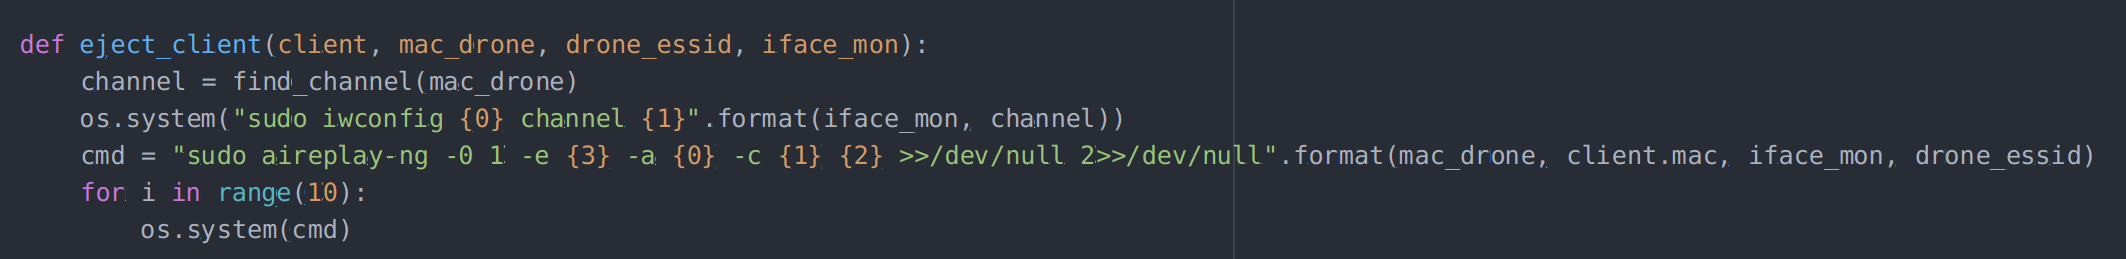
\includegraphics[scale=0.3]{images/aireplay.png}
  \caption{Utilisation d'\textbf{Aireplay} pour désauthentifier les clients}
\end{figure}

Une fois les clients désauthentifiés, nous nous reconnectons immédiatement au drone et sommes donc les premiers connectés au drone et les premiers à communiquer avec celui-ci donc "maître" du drone. Nous utilisons ensuite une application de contrôle via le navigateur web - disponible à l'adresse suivante: \url{https://github.com/functino/drone-browser} - afin de contrôler le drone avec le PC.

\subsection{Injection de paquets}
Cette seconde attaque a pour objectif d'injecter des commandes au drone sans en prendre le contrôle complètement.

\subsection{Exploitation d'une connexion Telnet}
La dernière attaque exploite une vulnérabilité du drone. Un service \textbf{Telnet} est ouvert et permet d'accéder à un shell \textbf{root} sur le drone.

\begin{figure}[H]
  \centering
  
\includegraphics[scale=0.3]{images/todo.png}
  \caption{Accès \textbf{Telnet root} sur l'ARDrone 2.0}
\end{figure}

Ainsi une fois connecté au réseau du drone, n'importe qui peut utiliser cette connexion \textbf{Telnet} pour être administrateur sur le drone. Une fois le shell \textbf{root} obtenu, on se retrouve avec un accès au système d'exploitation du drone, qui est un \textbf{Linux}, et il est possible de faire ce que l'on veut. L'attaquant peut alors réaliser une large variété d'attaques directement sur le système d'exploitation. Il peut interagir avec les processus qui tournent sur celui-ci et notamment le processus qui pilote le drone \textbf{AJOUTER NOM PROCESSUS}.

\begin{figure}[H]
  \centering
  
\includegraphics[scale=0.3]{images/todo.png}
  \caption{Processus s'exécutant sur l'ARDrone 2.0}
\end{figure}

Il ainsi possible de modifier n'importe quel fichier du système d'exploitation et de réaliser par exemple un Déni de service sur le drone depuis "l'intérieur" de celui-ci. Etant \textbf{root} sur le drone sans nécessité d'escalade de privilèges, nous cherchons ce qui serait le plus intéressant de faire avec ce contrôle du drone. Nous décidons de démontrer la possibilité d'implanter un virus sur le drone. Ainsi nous avons développé un script en bash qui sera envoyé sur le drone par l'application \textit{Krokmou} accompagné d'un fichier au choix de l'attaquant. L'envoi se fait via la connexion \textbf{FTP} au drone. Une fois les deux fichiers sur le drone, l'application utilise la connexion \textbf{Telnet} afin d'exécuter le script. Celui-ci se copie alors au sein du dossier \begin{verbatim}/bin\end{verbatim} du drone et s'ajoute à la liste des processus à lancer au démarrage du drone afin qu'il s'exécute en permanence sur le drone. Le script va alors régulièrement essayer de copier le fichier envoyé par l'attaquant avec le script sur une clé USB qui serait connectée au drone. L'utilisateur légitime peut utiliser une clé USB pour récupérer des vidéos filmées par le drone et enregistrées sur celle-ci. Par défaut et à des fins de démonstration, le script dépose sur les clés USBs connectées une image.

\begin{figure}[H]
  \centering
  
\includegraphics[scale=0.3]{images/todo.png}
  \caption{Dépose du virus et du fichier par l'application}
\end{figure}

Cette attaque démontre que le drone peut facilement servir de vecteur d'attaque pour diffuser un virus par clé USB.
